\documentclass[../../main.tex]{subfiles}
\begin{document}

\subsection*{8.4}
Tre fili conduttori sono tra loro paralleli e disposti ai vertici di un triangolo equilibrato di lato 2a=15cm.
\\Essi sono percorsi dalla stessa corrente i=10A corrente concorde all'asse x.
\\Calcolare il cmapo magnetico $\vec{B_c}$ nel centro C del triangolo e la forza F per unità di lunghezza sul filo disposto in P.
\\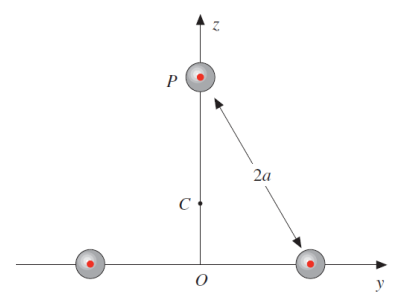
\includegraphics[scale=0.3]{e_8_4_0.png}
\\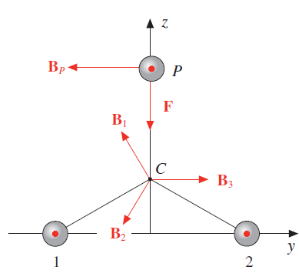
\includegraphics[scale=0.3]{e_8_4_1.png}
\subsubsection*{Formule utilizzate}
$\vec{B_p} = \frac{\mu_0 i \sqrt{3}}{4\pi a}\vec{u_x}$ per $z = a\sqrt{3}$
\subsubsection*{Soluzione punto a}
$\vec{B_1}+\vec{B_2}+\vec{B_3}=0$
\\$\vec{F}=i\int d\vec{g}\wedge\vec{B} = i\int dsB =iB\int ds$
\\$\vec{B_p} =\vec{B_1}+\vec{B_2}$
\\$\vec{B_c} = \vec{B_1}+\vec{B_2}+\vec{B_3}$ 
\subsubsection*{Soluzione punto b}
\newpage

\end{document}